\documentclass[12pt]{article}
\usepackage[spanish]{babel}
\usepackage[utf8]{inputenc}
\usepackage[margin=3cm]{geometry}
\usepackage{moreverb}
\usepackage[pdftex]{graphicx}
\usepackage{float}
\usepackage{mathtools}
\usepackage{fancyvrb}
\usepackage{color}
\usepackage[math]{iwona}
\usepackage[T1]{fontenc}

\title{\begin{Huge} Redes de Computadores\\
Tarea 3 \\
No somos nada, ¡Hola Internet! (Capa de Red)\end{Huge}}
\author{
\\\\\\\\\textbf{Integrantes}:\\
\begin{tabular}{cc}
	Guillermo Fernández & Álvaro Rojas \\
	guillermo.fernanb.12@alumnos.usm.cl & alvaro.rojasv@alumnos.usm.cl \\
	201073523-0 & 201073555-9 \\
\end{tabular}
\\\\\\\\\textbf{Profesor:}\\
Oscar Encina
\\\\\\ \textbf{Ayudantes:}\\
Alex Arenas\\
Carlos Marchant\\\\\\}
\date{02 de Junio, 2014}

\begin{document}

\maketitle
\newpage
\pagebreak

\section{Introducción}
En este laboratorio, se analizará qué es lo que ocurre con los paquetes a medida que viajan por la gran red de redes que supone Internet, y además, se conocerá cómo funciona el algoritmo vector-distancia con el que los routers completan sus tablas de costos.

\subsection{Objetivos}
\begin{itemize}
\item {\it Evidenciar la real dimensión de la internet y analizar su interconexión.}
\item {\it Conocer el funcionamiento del algoritmo de enrutamiento llamado \emph{Algoritmo de Vector-Distancia}.}
\item {\it Recordar la programación en Python.}
\end{itemize}

\newpage

\section{Desarrollo}
\subsection{Las dimensiones de Internet}
En esta sección, se han analizado una serie de sitios web que, mediante el ingreso de sus URL al programa \textit{Open Visual Traceroute}, se puede conocer qué camino toman los paquetes a través del planeta, evidenciándose así que existen saltos tan extraordinarios como lo que significa ir de un continente a otro. Los sitios web analizados son los siguientes:

\begin{enumerate}
\item {\it http://moodle.inf.utfsm.cl/}
\item {\it http://google.cl/}
\item {\it http://cime.cl/}
\item {\it http://wikipedia.com/}
\item {\it http://www.chile.embassy.gov.au/}
\end{enumerate}

Para realizarlo, se ejecuta el código de la siguiente forma. En primer lugar, se ejecuta \emph{servidorTCP.java}:

\begin{figure}[H] 
\centering 
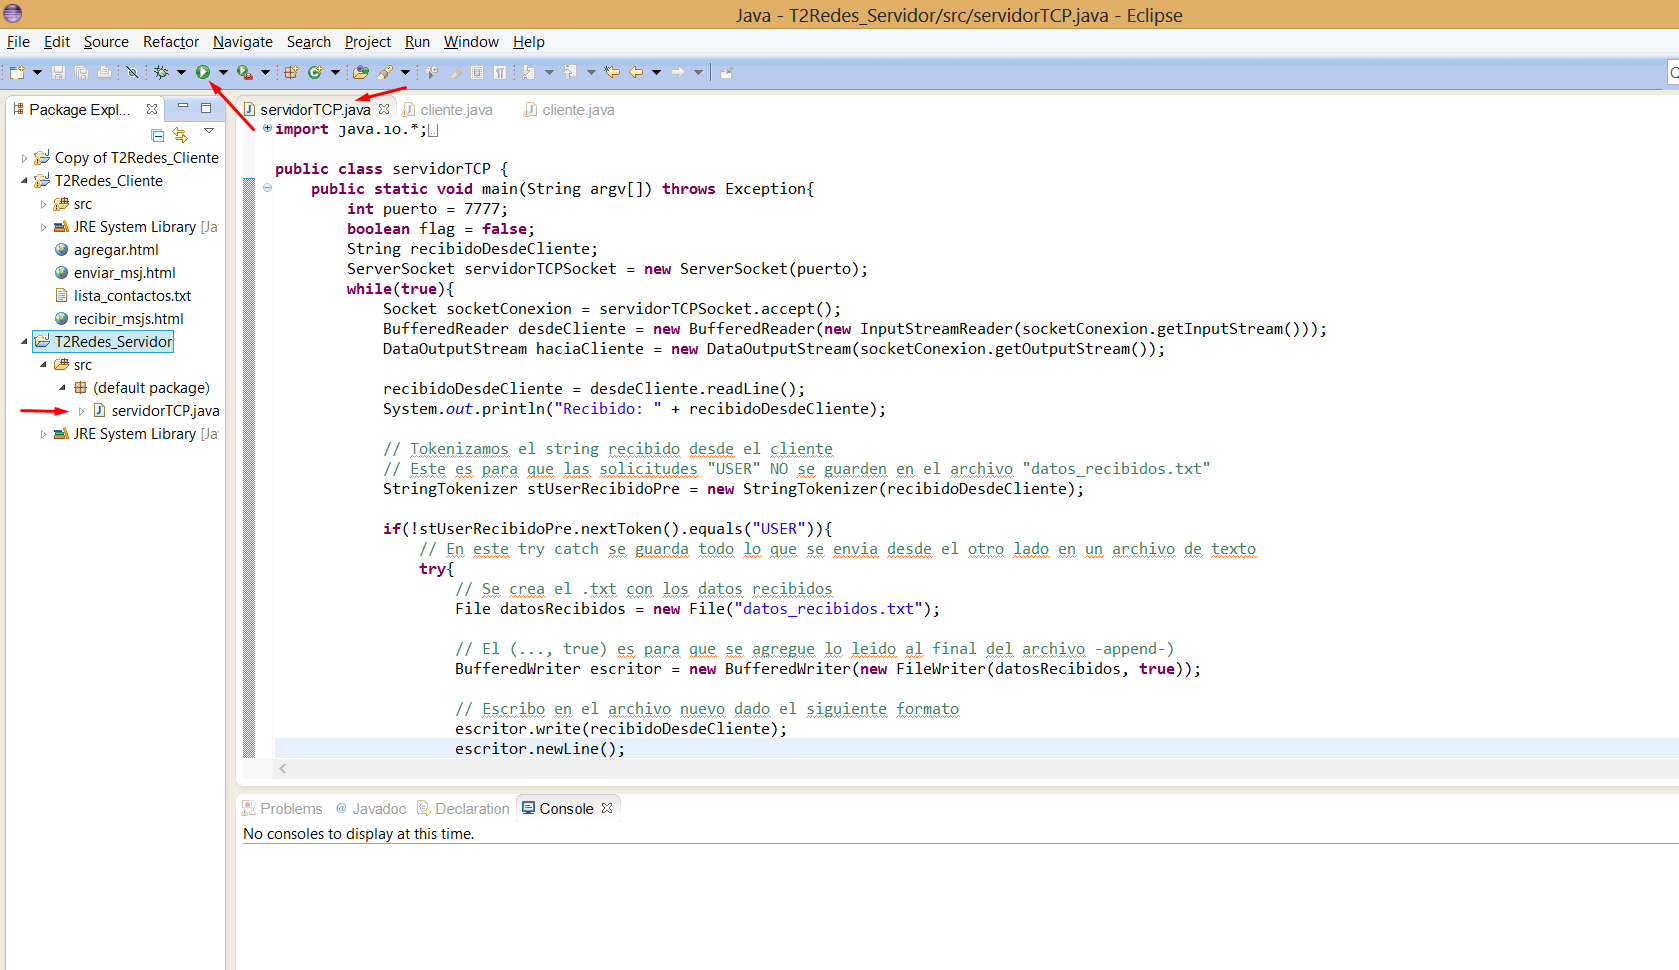
\includegraphics[width=1\textwidth]{imagenes/1.png} \caption{\small \textbf{Iniciando servidor}} 
\label{fig:diagrama_1} 
\end{figure}

Se escogió un servidor con protocolos TCP en vez de UDP debido a que se busca la integridad de los mensajes y archivos enviados.\\

Luego, se inician los dos clientes con diferentes puertos entre ellos y con el servidor:\\

De esta forma, posteriormente se puede acceder a mandar solicitudes de conexión y aceptarlas para poder mandar mensajes entre clientes a través del servidor TCP.

\subsection{Conectar ambos clientes}

Mediante la agregación de contactos realizado en la Tarea 1, los clientes quedan ''conectados'' además de registrados en la lista de contactos.\\

\subsection{Captura de paquetes con Wireshark}

Mediante la herramienta RawCap, que permite monitorear interfaces loopback (dado que se utilizó solo un computador para la ejecución, lo que quiere decir que el envío de mensajes es entre localhost y localhost) y permite generar un archivo \emph{.pcap} que Wireshark puede leer, se puede generar un registro de los paquetes transferidos, y luego ser visualizados con Wireshark:

\subsection{Enviar un mensaje entre clientes}

Para enviar un mensaje entre clientes, se identifica quien es el usuario emisor, y a quién va dirigido el mensaje, además del mensaje propiamente tal.

El otro cliente tiene la posibilidad de ver los mensajes recibidos mediante la opción habilitada en la página.

\subsection{Enviar una respuesta entre clientes}

Para enviar una respuesta entre clientes, se identifica quien es el usuario, y a quién va dirigida la respuesta, además del mensaje propiamente tal.

El otro cliente tiene la posibilidad de ver las respuestas recibidos mediante la opción habilitada en la página.\\

\subsection{Mostrar en Wireshark los mensajes enviados}
En la figura 11, se observan los números de puertos de origen y de destino de los paquetes enviados. En el caso del puerto de origen, se ve que corresponde al 65172. Este puerto correspondería a un socket perteneciente al puerto 6666 que se ha definido en el código Java. El número 7777 corresponde al puerto en el que está escuchando el servidor TCP.\\

El socket asociado al puerto de cliente no tiene por qué ser el mismo, ya que a medida que se hace la transferencia de paquetes, el socket asociado a los puertos de cliente va cambiando, tal como se verá en la siguiente captura.\\

En la figura 12 se puede observar un mensaje desde el servidor al cliente; en este caso, el puerto de origen es el del servidor que es el 7777, y el de destino es 65181, que vendría a ser un socket asentado en el puerto 6666 que se definió en el código Java para el cliente.\\

Además, en esta imagen se pueden observar las IP de origen y destino de los paquetes, que en este caso son ambas iguales a 127.0.0.1, ya que el envío de mensajes se hizo en el mismo computador, o sea, desde \emph{localhost} a \emph{localhost}.

En cuando a los números de secuencia y ACK's, en TCP se relacionan con la transferencia de datos fiable. Los números de secuencia, corresponden al primer byte numerado de cada segmento, y el ACK es el número de secuencia del siguiente byte que el otro host está esperando por recibir. En este sentido, al comienzo de la transmisión de paquetes, la primera señal que se envía es un SYN (sincronización de números de secuencia), y luego se puede observar que en el caso de envío desde cliente a servidor, el número de secuencia  va tomando el mismo valor del ACK anterior, mientras que el ACK toma el valor 1. Cuando el envío es desde servidor a cliente, ahora el número de secuencia es 1 y el ACK es uno más el mismo número de secuencia del envío servidor-cliente. Cabe destacar que la señal PSH quiere decir que no se ha esperado que el buffer se llene para enviar, sino que el paquete se envió de inmediato.

\newpage

\subsection{Diagramas de conexiones con los puertos, sockets e IP's}
El resultado del análisis del punto 2.6 usando \emph{Wireshark} es:\\

\end{document}